\documentclass{report}

\usepackage[a4paper,margin=0.5in]{geometry}
\usepackage{array}
\usepackage{xcolor}
\usepackage{graphicx}
\usepackage{float}
\usepackage{adjustbox}

\newcolumntype{P}[1]{>{\raggedleft\arraybackslash}b{#1}}
\newcommand{\bftab}{\fontseries{b}\selectfont}

\begin{document}
\section{Plots of single attributes}

\subsection{residual sugar}
\begin{figure}[H]
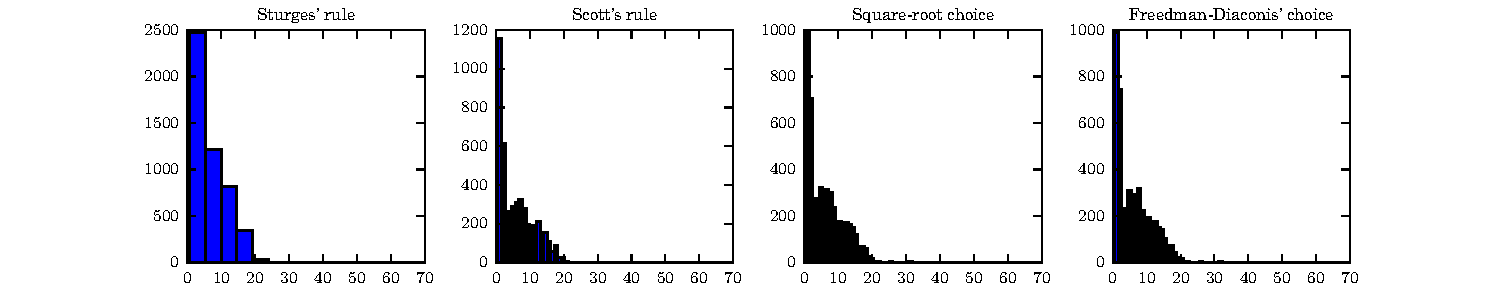
\includegraphics[width=\textwidth]{histograms/residual_sugar.pdf}
\caption{Histograms of attribute \emph{residual sugar} using different binning methods}\end{figure}

\begin{figure}[H]
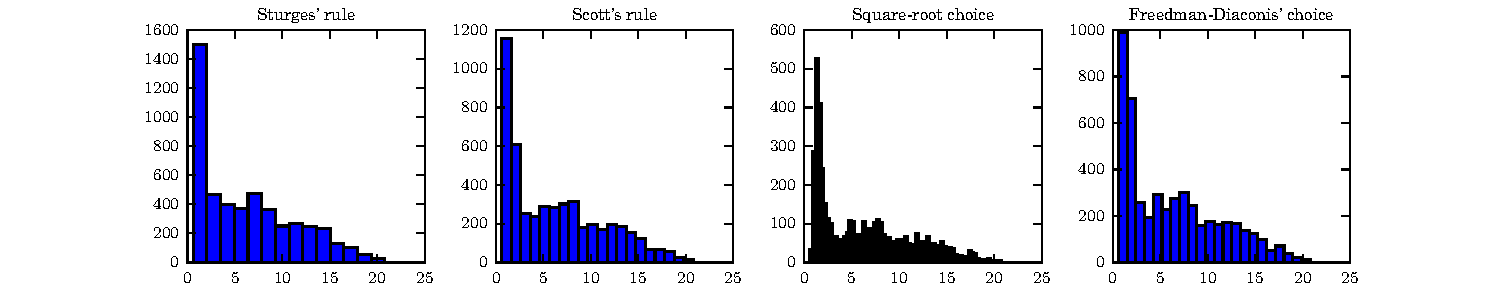
\includegraphics[width=\textwidth]{histograms/residual_sugar_filtered.pdf}
\caption{Histograms of attribute \emph{residual sugar} with outliers further than 3 standard deviations from the mean filtered}
\end{figure}

\begin{figure}[H]
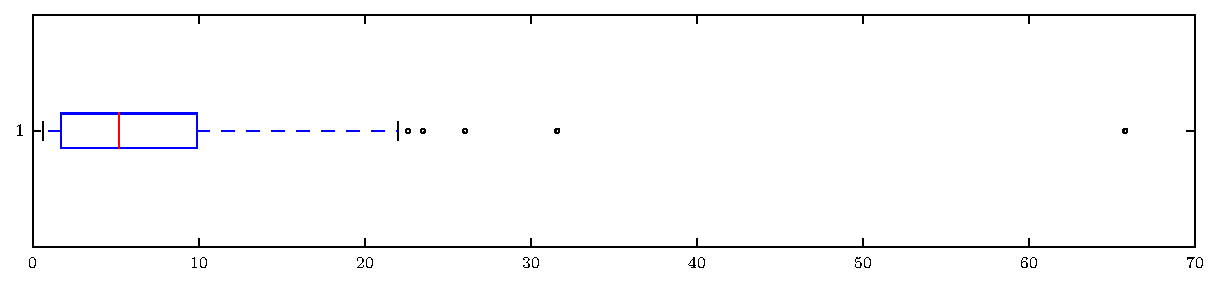
\includegraphics[width=\textwidth]{boxplots/residual_sugar.pdf}
\caption{Boxplot of attribute \emph{residual sugar}}\end{figure}

\newpage\subsection{fixed acidity}
\begin{figure}[H]
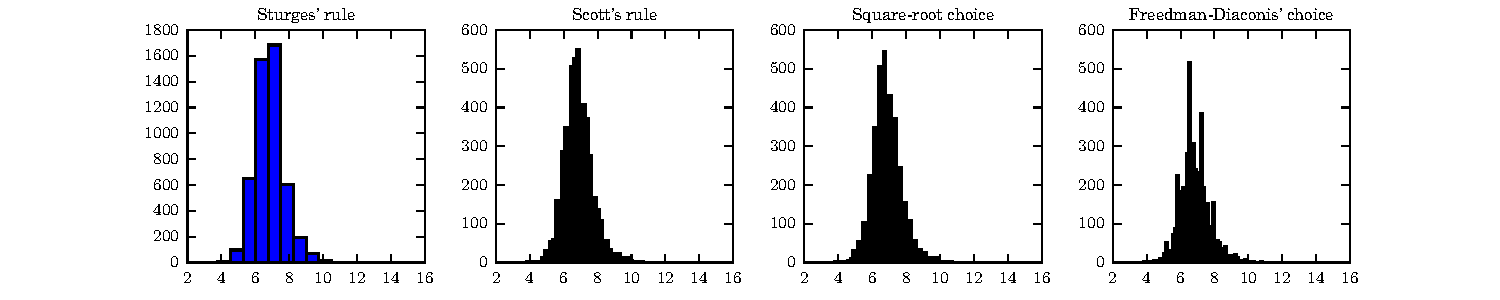
\includegraphics[width=\textwidth]{histograms/fixed_acidity.pdf}
\caption{Histograms of attribute \emph{fixed acidity} using different binning methods}\end{figure}

\begin{figure}[H]
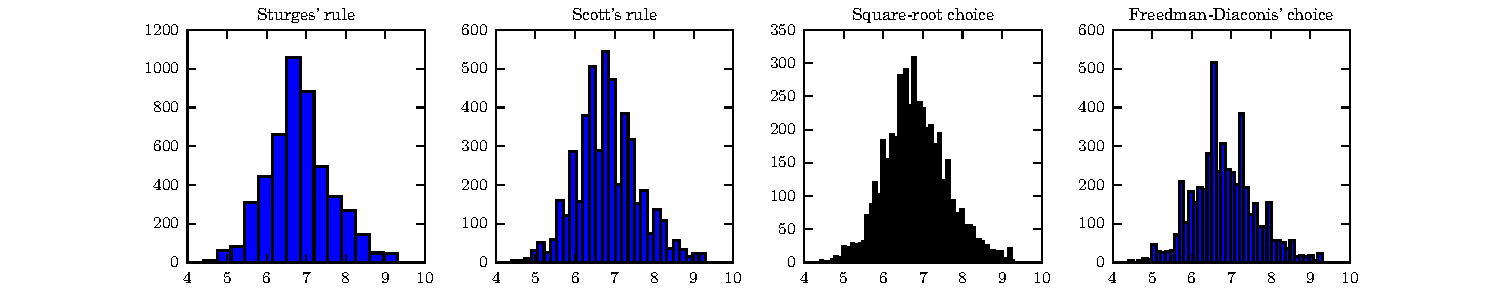
\includegraphics[width=\textwidth]{histograms/fixed_acidity_filtered.pdf}
\caption{Histograms of attribute \emph{fixed acidity} with outliers further than 3 standard deviations from the mean filtered}
\end{figure}

\begin{figure}[H]
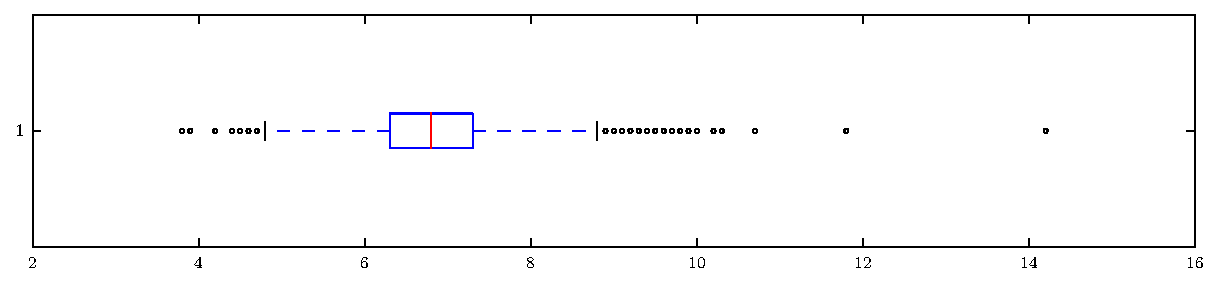
\includegraphics[width=\textwidth]{boxplots/fixed_acidity.pdf}
\caption{Boxplot of attribute \emph{fixed acidity}}\end{figure}

\newpage\subsection{density}
\begin{figure}[H]
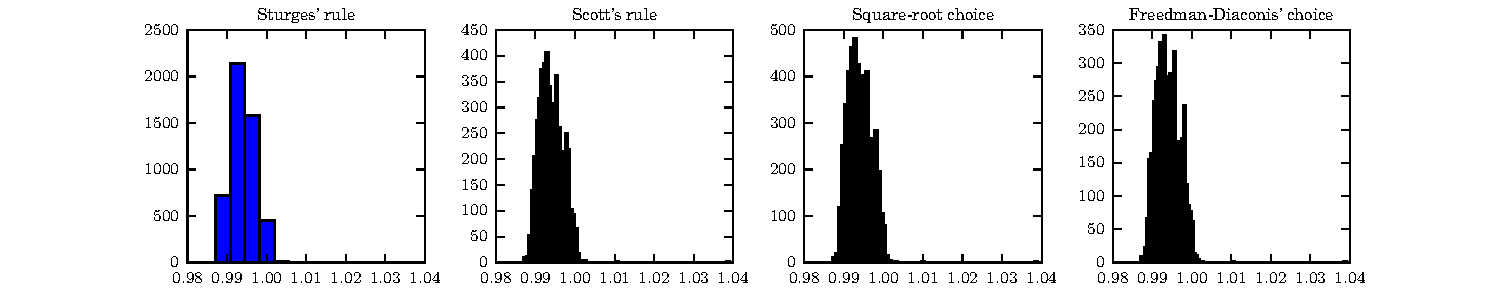
\includegraphics[width=\textwidth]{histograms/density.pdf}
\caption{Histograms of attribute \emph{density} using different binning methods}\end{figure}

\begin{figure}[H]
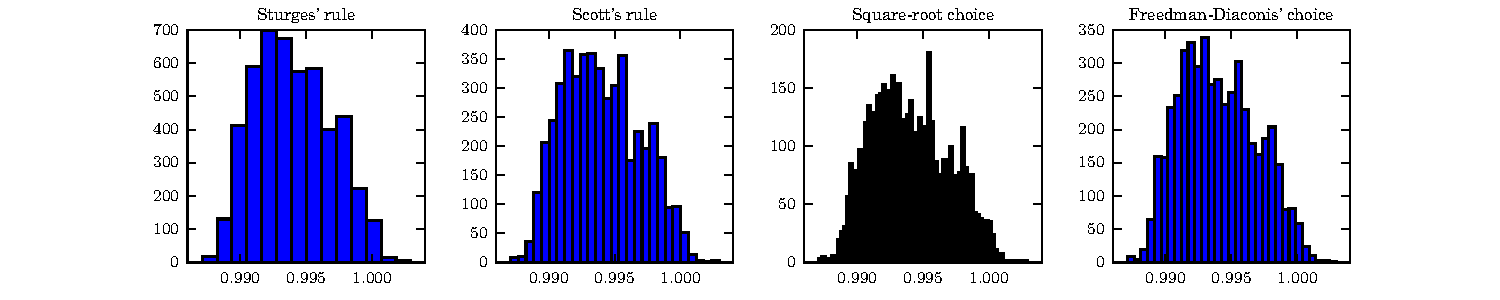
\includegraphics[width=\textwidth]{histograms/density_filtered.pdf}
\caption{Histograms of attribute \emph{density} with outliers further than 3 standard deviations from the mean filtered}
\end{figure}

\begin{figure}[H]
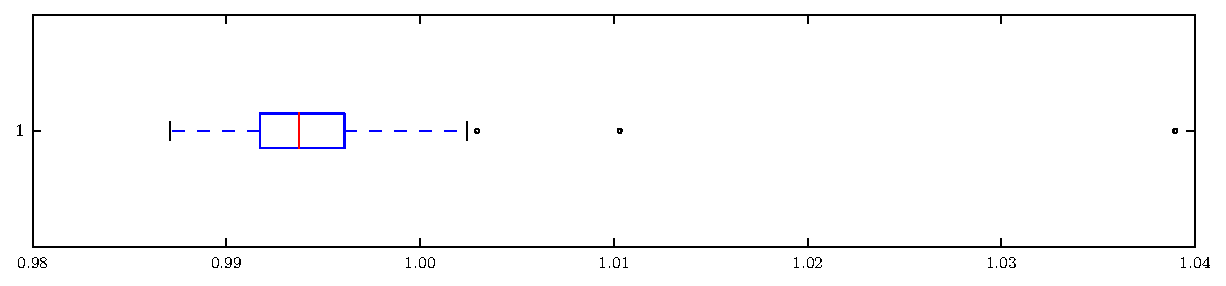
\includegraphics[width=\textwidth]{boxplots/density.pdf}
\caption{Boxplot of attribute \emph{density}}\end{figure}

\newpage\subsection{volatile acidity}
\begin{figure}[H]
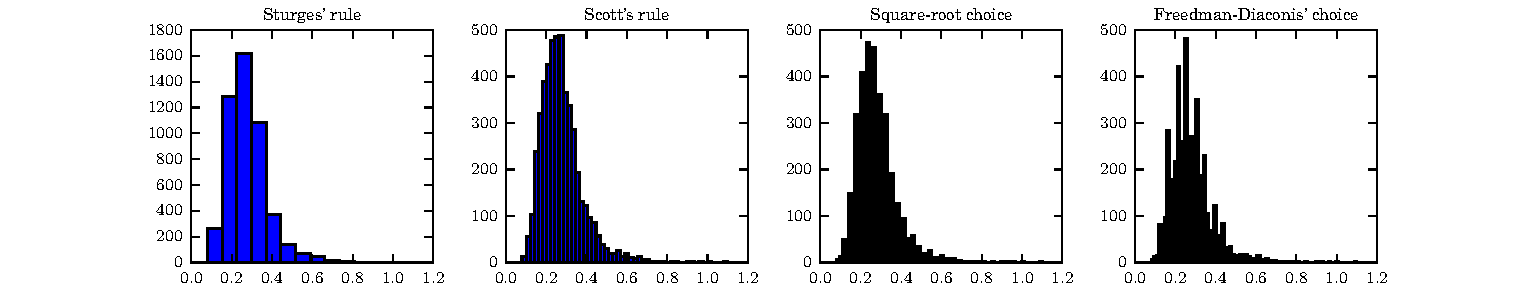
\includegraphics[width=\textwidth]{histograms/volatile_acidity.pdf}
\caption{Histograms of attribute \emph{volatile acidity} using different binning methods}\end{figure}

\begin{figure}[H]
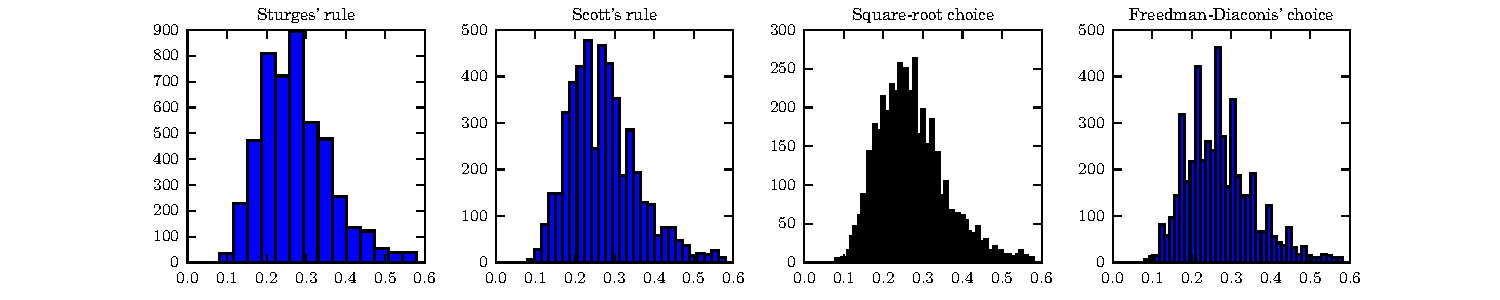
\includegraphics[width=\textwidth]{histograms/volatile_acidity_filtered.pdf}
\caption{Histograms of attribute \emph{volatile acidity} with outliers further than 3 standard deviations from the mean filtered}
\end{figure}

\begin{figure}[H]
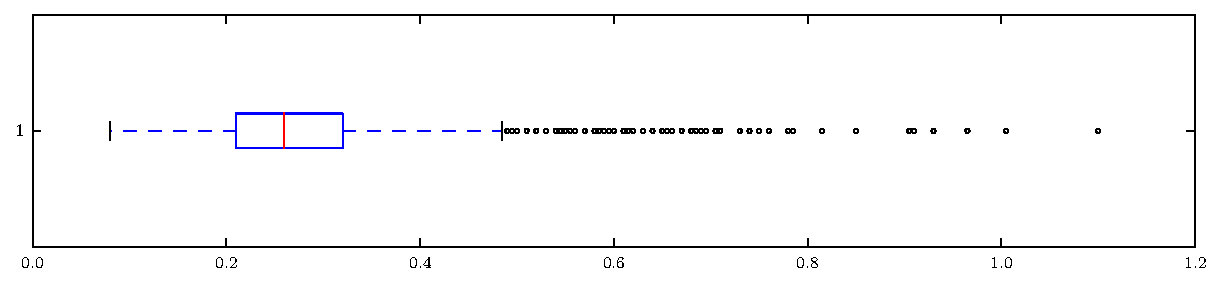
\includegraphics[width=\textwidth]{boxplots/volatile_acidity.pdf}
\caption{Boxplot of attribute \emph{volatile acidity}}\end{figure}

\newpage\subsection{total sulfur dioxide}
\begin{figure}[H]
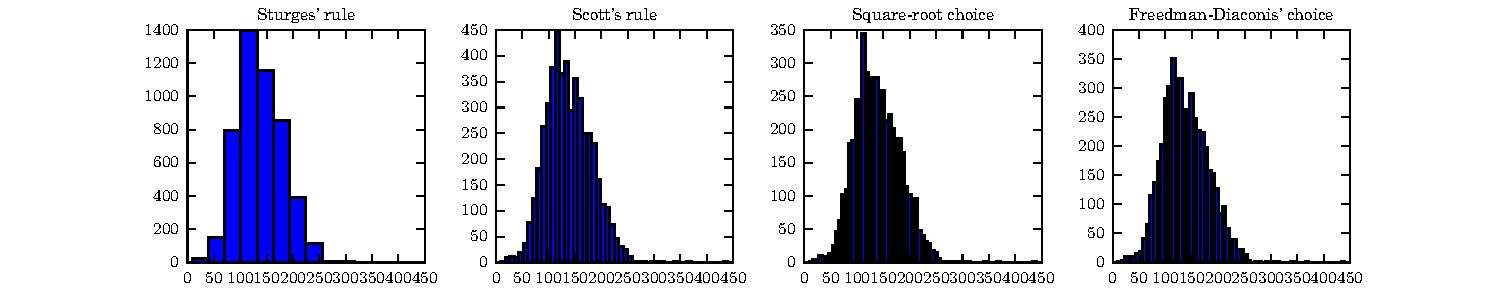
\includegraphics[width=\textwidth]{histograms/total_sulfur_dioxide.pdf}
\caption{Histograms of attribute \emph{total sulfur dioxide} using different binning methods}\end{figure}

\begin{figure}[H]
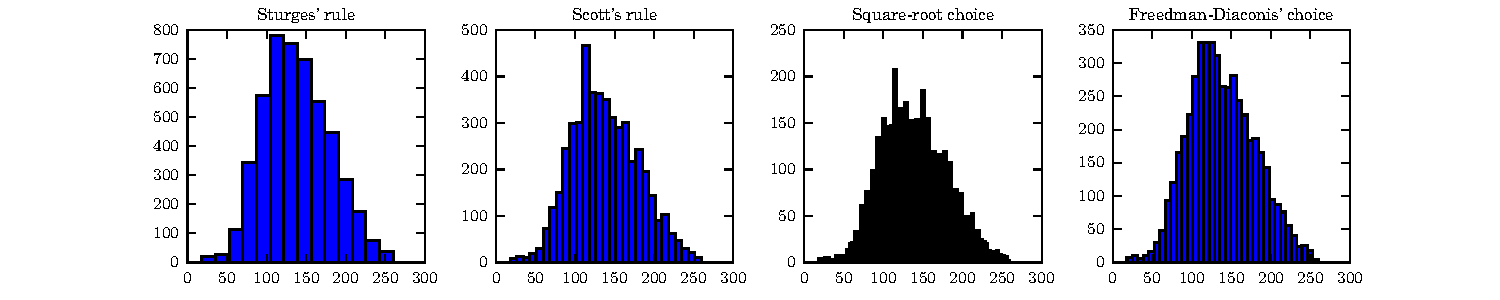
\includegraphics[width=\textwidth]{histograms/total_sulfur_dioxide_filtered.pdf}
\caption{Histograms of attribute \emph{total sulfur dioxide} with outliers further than 3 standard deviations from the mean filtered}
\end{figure}

\begin{figure}[H]
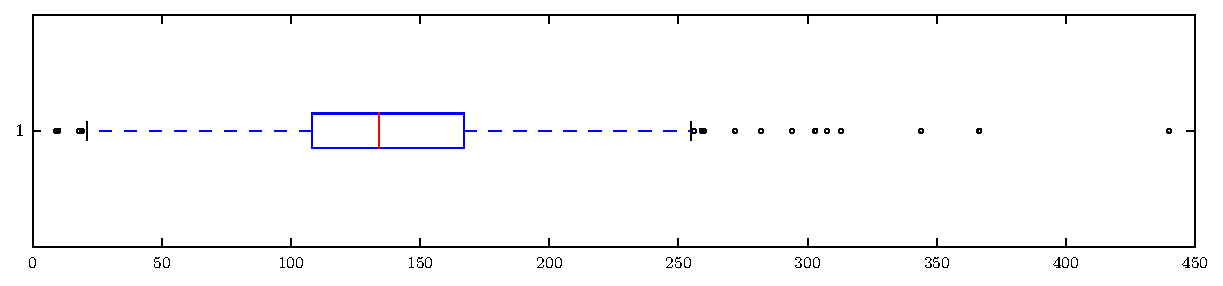
\includegraphics[width=\textwidth]{boxplots/total_sulfur_dioxide.pdf}
\caption{Boxplot of attribute \emph{total sulfur dioxide}}\end{figure}

\newpage\subsection{alcohol}
\begin{figure}[H]
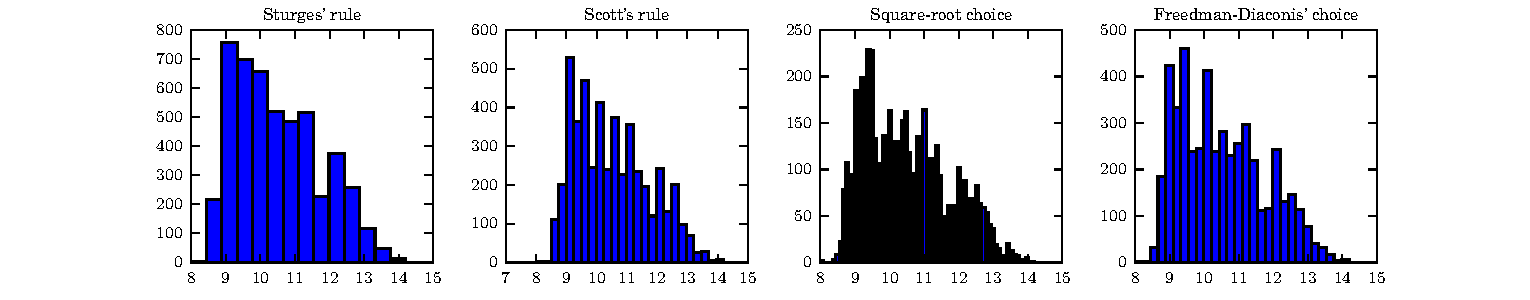
\includegraphics[width=\textwidth]{histograms/alcohol.pdf}
\caption{Histograms of attribute \emph{alcohol} using different binning methods}\end{figure}

\begin{figure}[H]
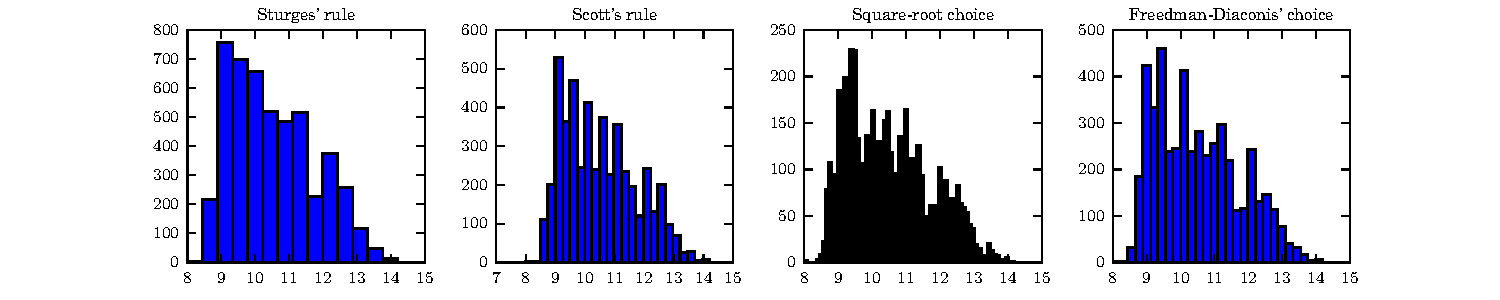
\includegraphics[width=\textwidth]{histograms/alcohol_filtered.pdf}
\caption{Histograms of attribute \emph{alcohol} with outliers further than 3 standard deviations from the mean filtered}
\end{figure}

\begin{figure}[H]
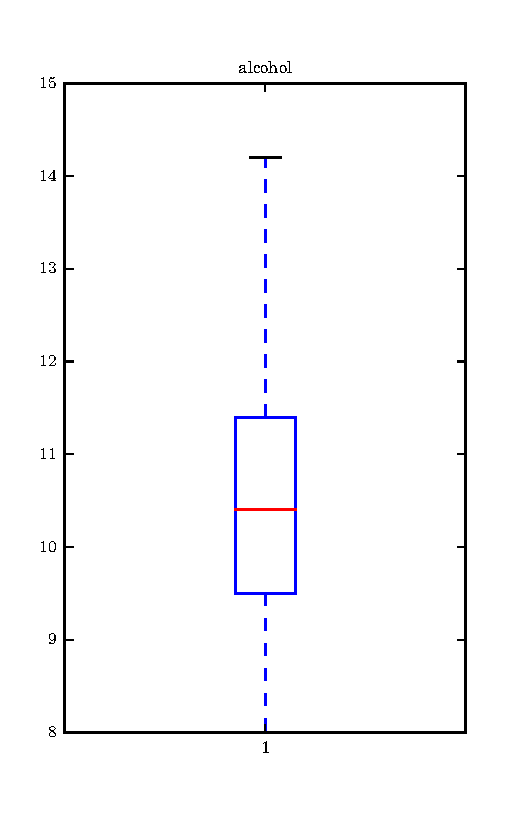
\includegraphics[width=\textwidth]{boxplots/alcohol.pdf}
\caption{Boxplot of attribute \emph{alcohol}}\end{figure}

\newpage\subsection{quality}
\begin{figure}[H]
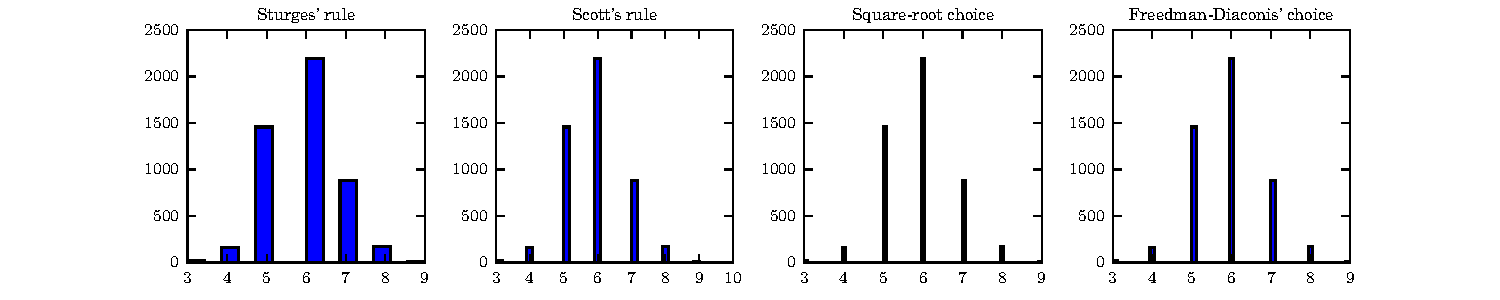
\includegraphics[width=\textwidth]{histograms/quality.pdf}
\caption{Histograms of attribute \emph{quality} using different binning methods}\end{figure}

\begin{figure}[H]
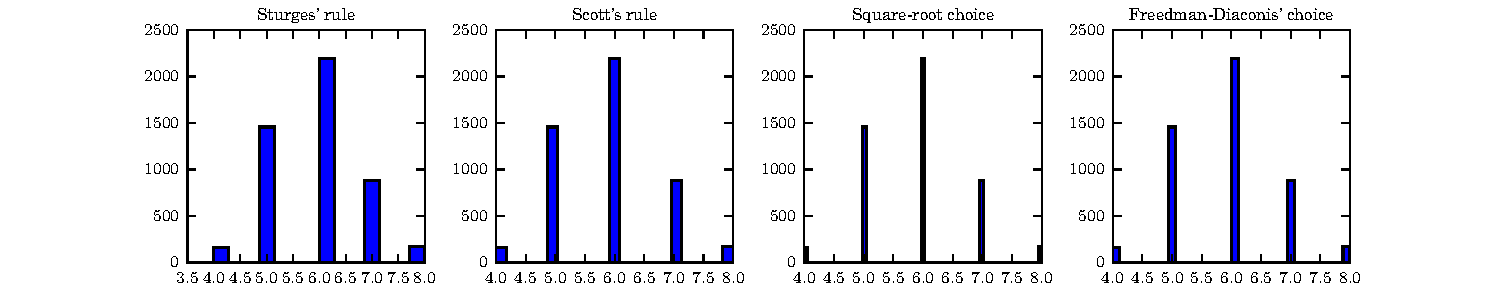
\includegraphics[width=\textwidth]{histograms/quality_filtered.pdf}
\caption{Histograms of attribute \emph{quality} with outliers further than 3 standard deviations from the mean filtered}
\end{figure}

\begin{figure}[H]
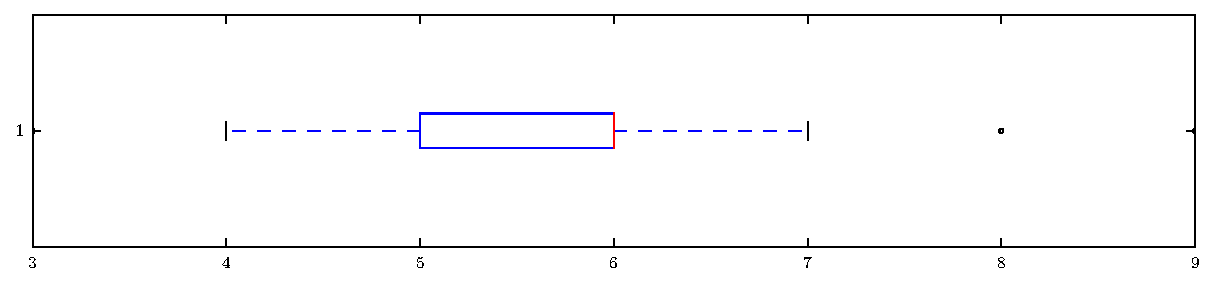
\includegraphics[width=\textwidth]{boxplots/quality.pdf}
\caption{Boxplot of attribute \emph{quality}}\end{figure}

\newpage\subsection{sulphates}
\begin{figure}[H]
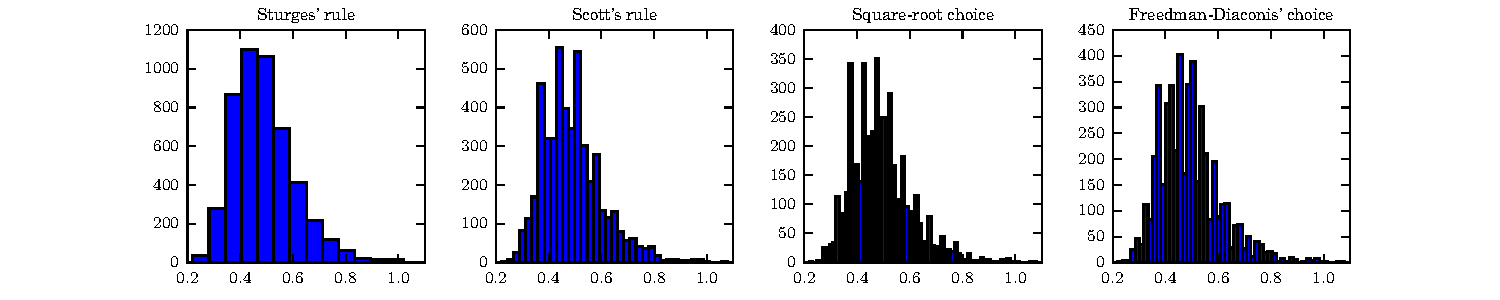
\includegraphics[width=\textwidth]{histograms/sulphates.pdf}
\caption{Histograms of attribute \emph{sulphates} using different binning methods}\end{figure}

\begin{figure}[H]
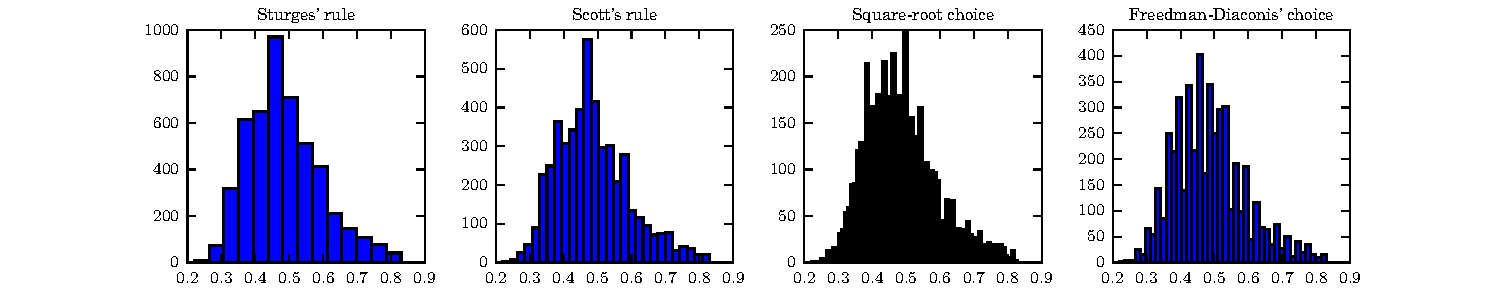
\includegraphics[width=\textwidth]{histograms/sulphates_filtered.pdf}
\caption{Histograms of attribute \emph{sulphates} with outliers further than 3 standard deviations from the mean filtered}
\end{figure}

\begin{figure}[H]
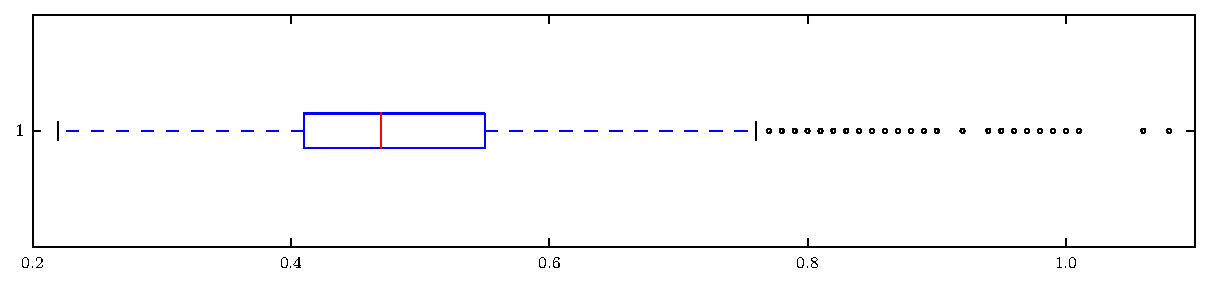
\includegraphics[width=\textwidth]{boxplots/sulphates.pdf}
\caption{Boxplot of attribute \emph{sulphates}}\end{figure}

\newpage\subsection{free sulfur dioxide}
\begin{figure}[H]
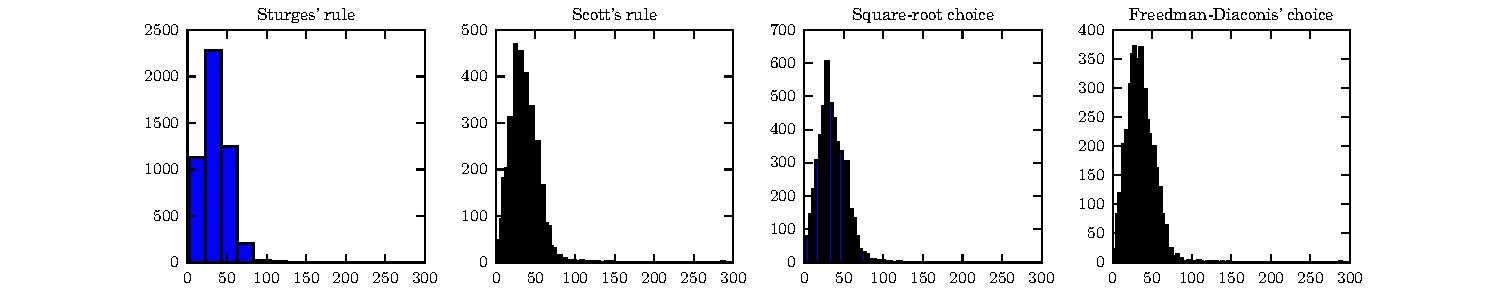
\includegraphics[width=\textwidth]{histograms/free_sulfur_dioxide.pdf}
\caption{Histograms of attribute \emph{free sulfur dioxide} using different binning methods}\end{figure}

\begin{figure}[H]
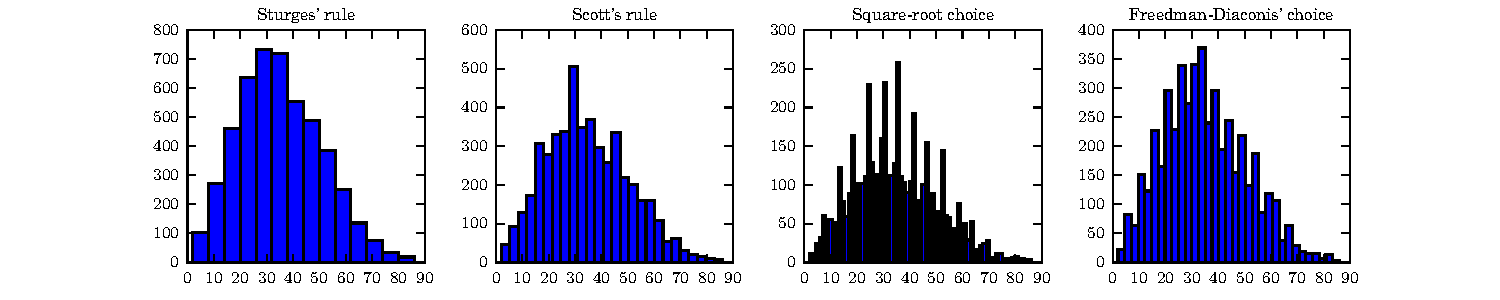
\includegraphics[width=\textwidth]{histograms/free_sulfur_dioxide_filtered.pdf}
\caption{Histograms of attribute \emph{free sulfur dioxide} with outliers further than 3 standard deviations from the mean filtered}
\end{figure}

\begin{figure}[H]
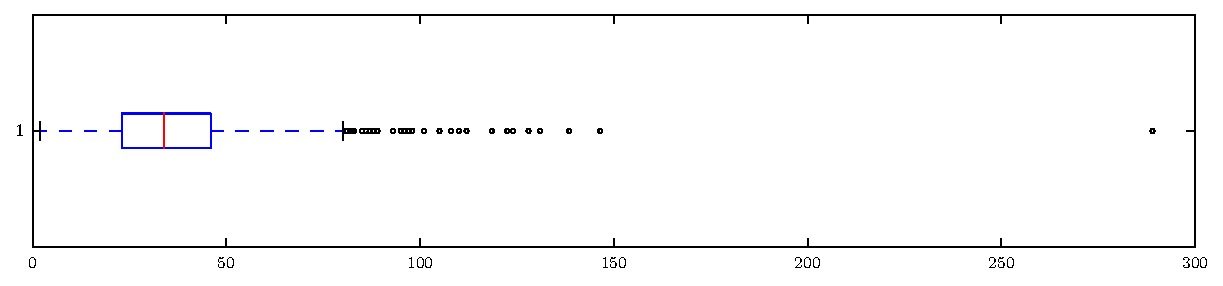
\includegraphics[width=\textwidth]{boxplots/free_sulfur_dioxide.pdf}
\caption{Boxplot of attribute \emph{free sulfur dioxide}}\end{figure}

\newpage\subsection{chlorides}
\begin{figure}[H]
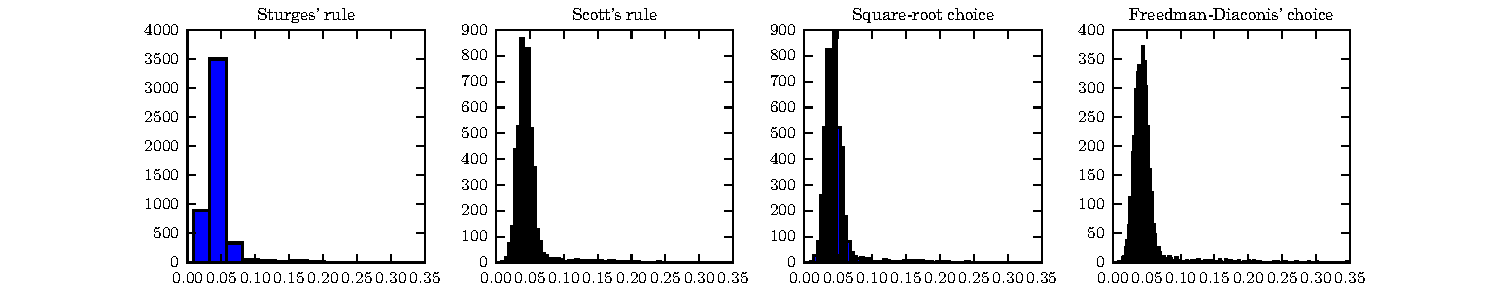
\includegraphics[width=\textwidth]{histograms/chlorides.pdf}
\caption{Histograms of attribute \emph{chlorides} using different binning methods}\end{figure}

\begin{figure}[H]
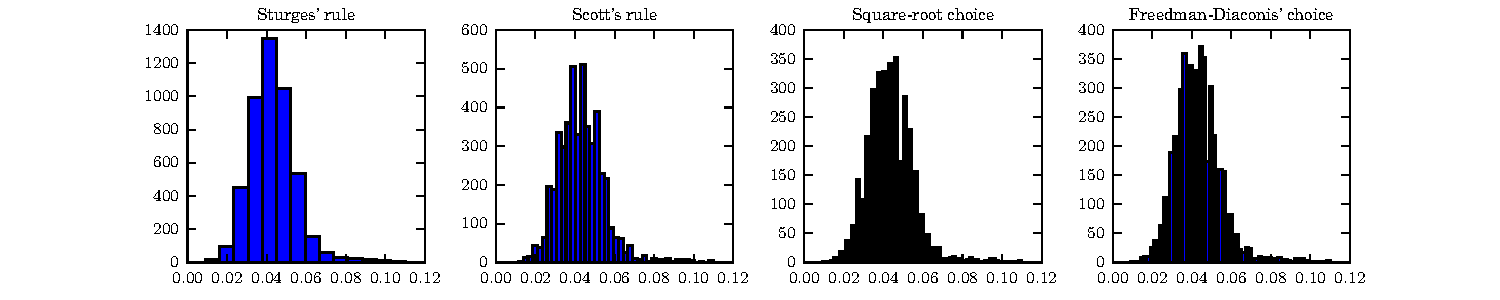
\includegraphics[width=\textwidth]{histograms/chlorides_filtered.pdf}
\caption{Histograms of attribute \emph{chlorides} with outliers further than 3 standard deviations from the mean filtered}
\end{figure}

\begin{figure}[H]
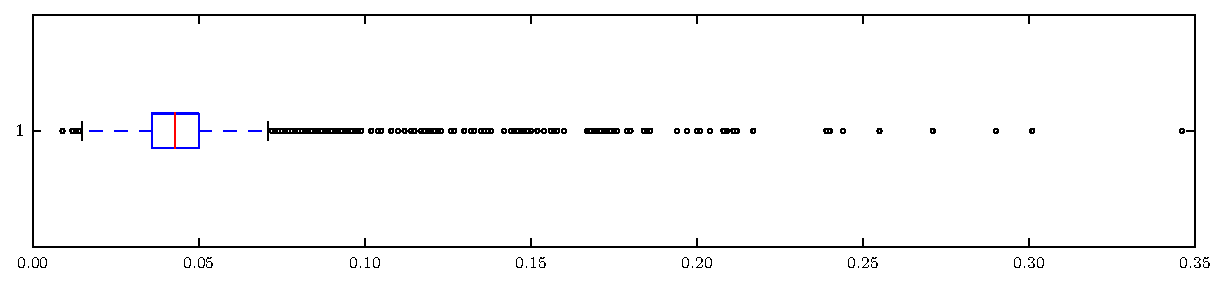
\includegraphics[width=\textwidth]{boxplots/chlorides.pdf}
\caption{Boxplot of attribute \emph{chlorides}}\end{figure}

\newpage\subsection{citric acid}
\begin{figure}[H]
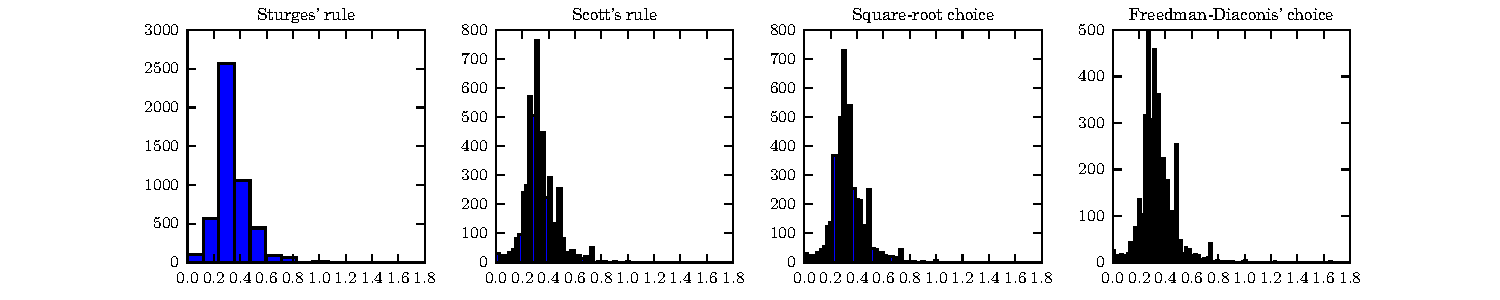
\includegraphics[width=\textwidth]{histograms/citric_acid.pdf}
\caption{Histograms of attribute \emph{citric acid} using different binning methods}\end{figure}

\begin{figure}[H]
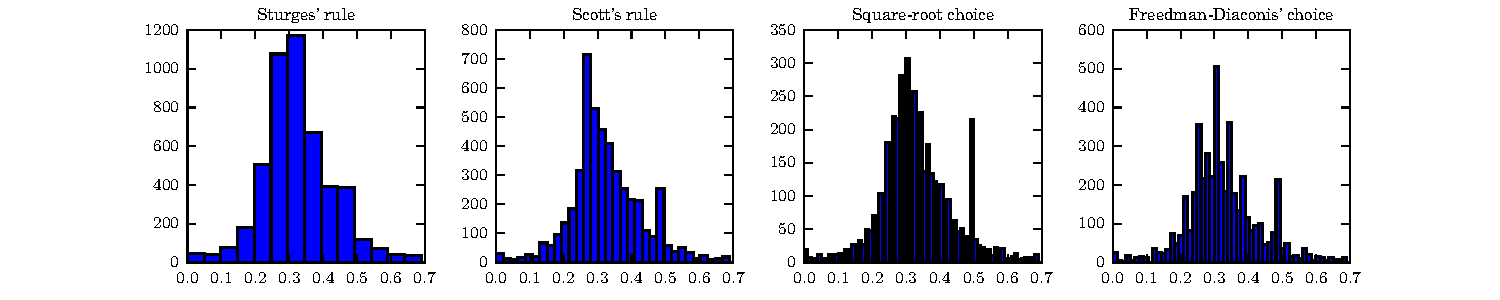
\includegraphics[width=\textwidth]{histograms/citric_acid_filtered.pdf}
\caption{Histograms of attribute \emph{citric acid} with outliers further than 3 standard deviations from the mean filtered}
\end{figure}

\begin{figure}[H]
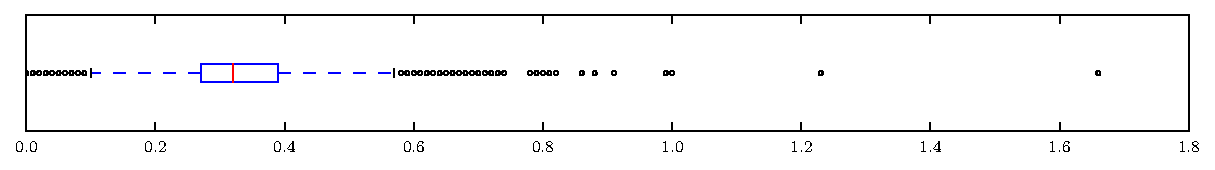
\includegraphics[width=\textwidth]{boxplots/citric_acid.pdf}
\caption{Boxplot of attribute \emph{citric acid}}\end{figure}

\newpage\subsection{pH}
\begin{figure}[H]
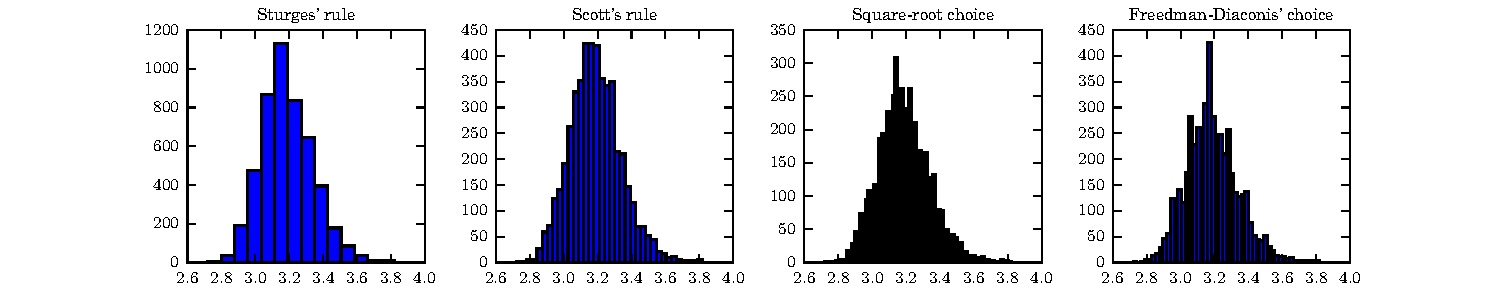
\includegraphics[width=\textwidth]{histograms/pH.pdf}
\caption{Histograms of attribute \emph{pH} using different binning methods}\end{figure}

\begin{figure}[H]
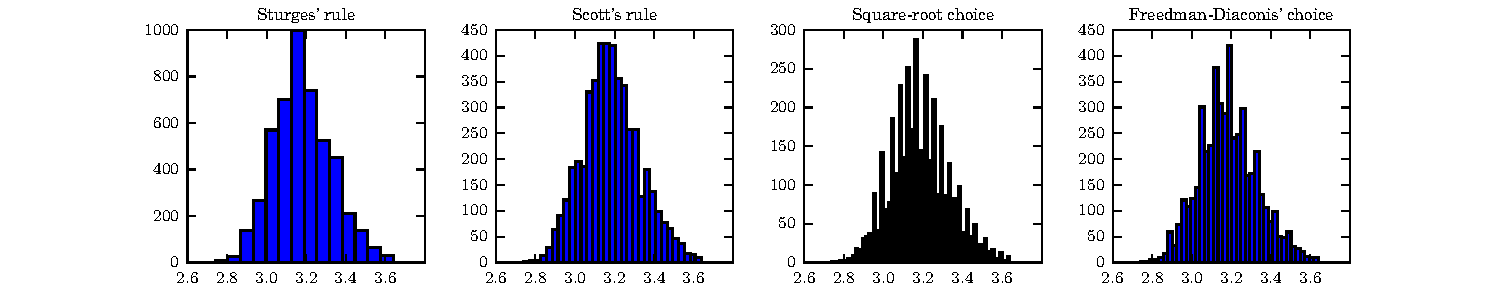
\includegraphics[width=\textwidth]{histograms/pH_filtered.pdf}
\caption{Histograms of attribute \emph{pH} with outliers further than 3 standard deviations from the mean filtered}
\end{figure}

\begin{figure}[H]
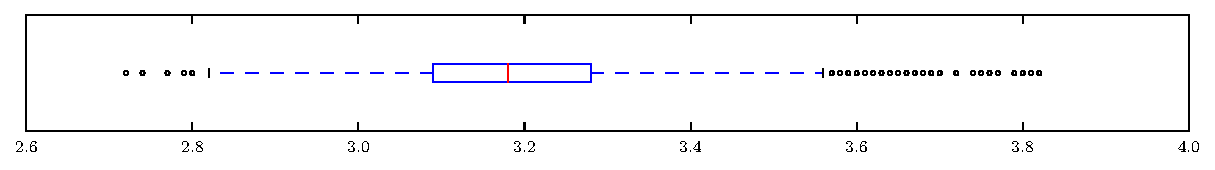
\includegraphics[width=\textwidth]{boxplots/pH.pdf}
\caption{Boxplot of attribute \emph{pH}}\end{figure}

\newpage\section{Plots for the whole feature set}

\begin{figure}[H]
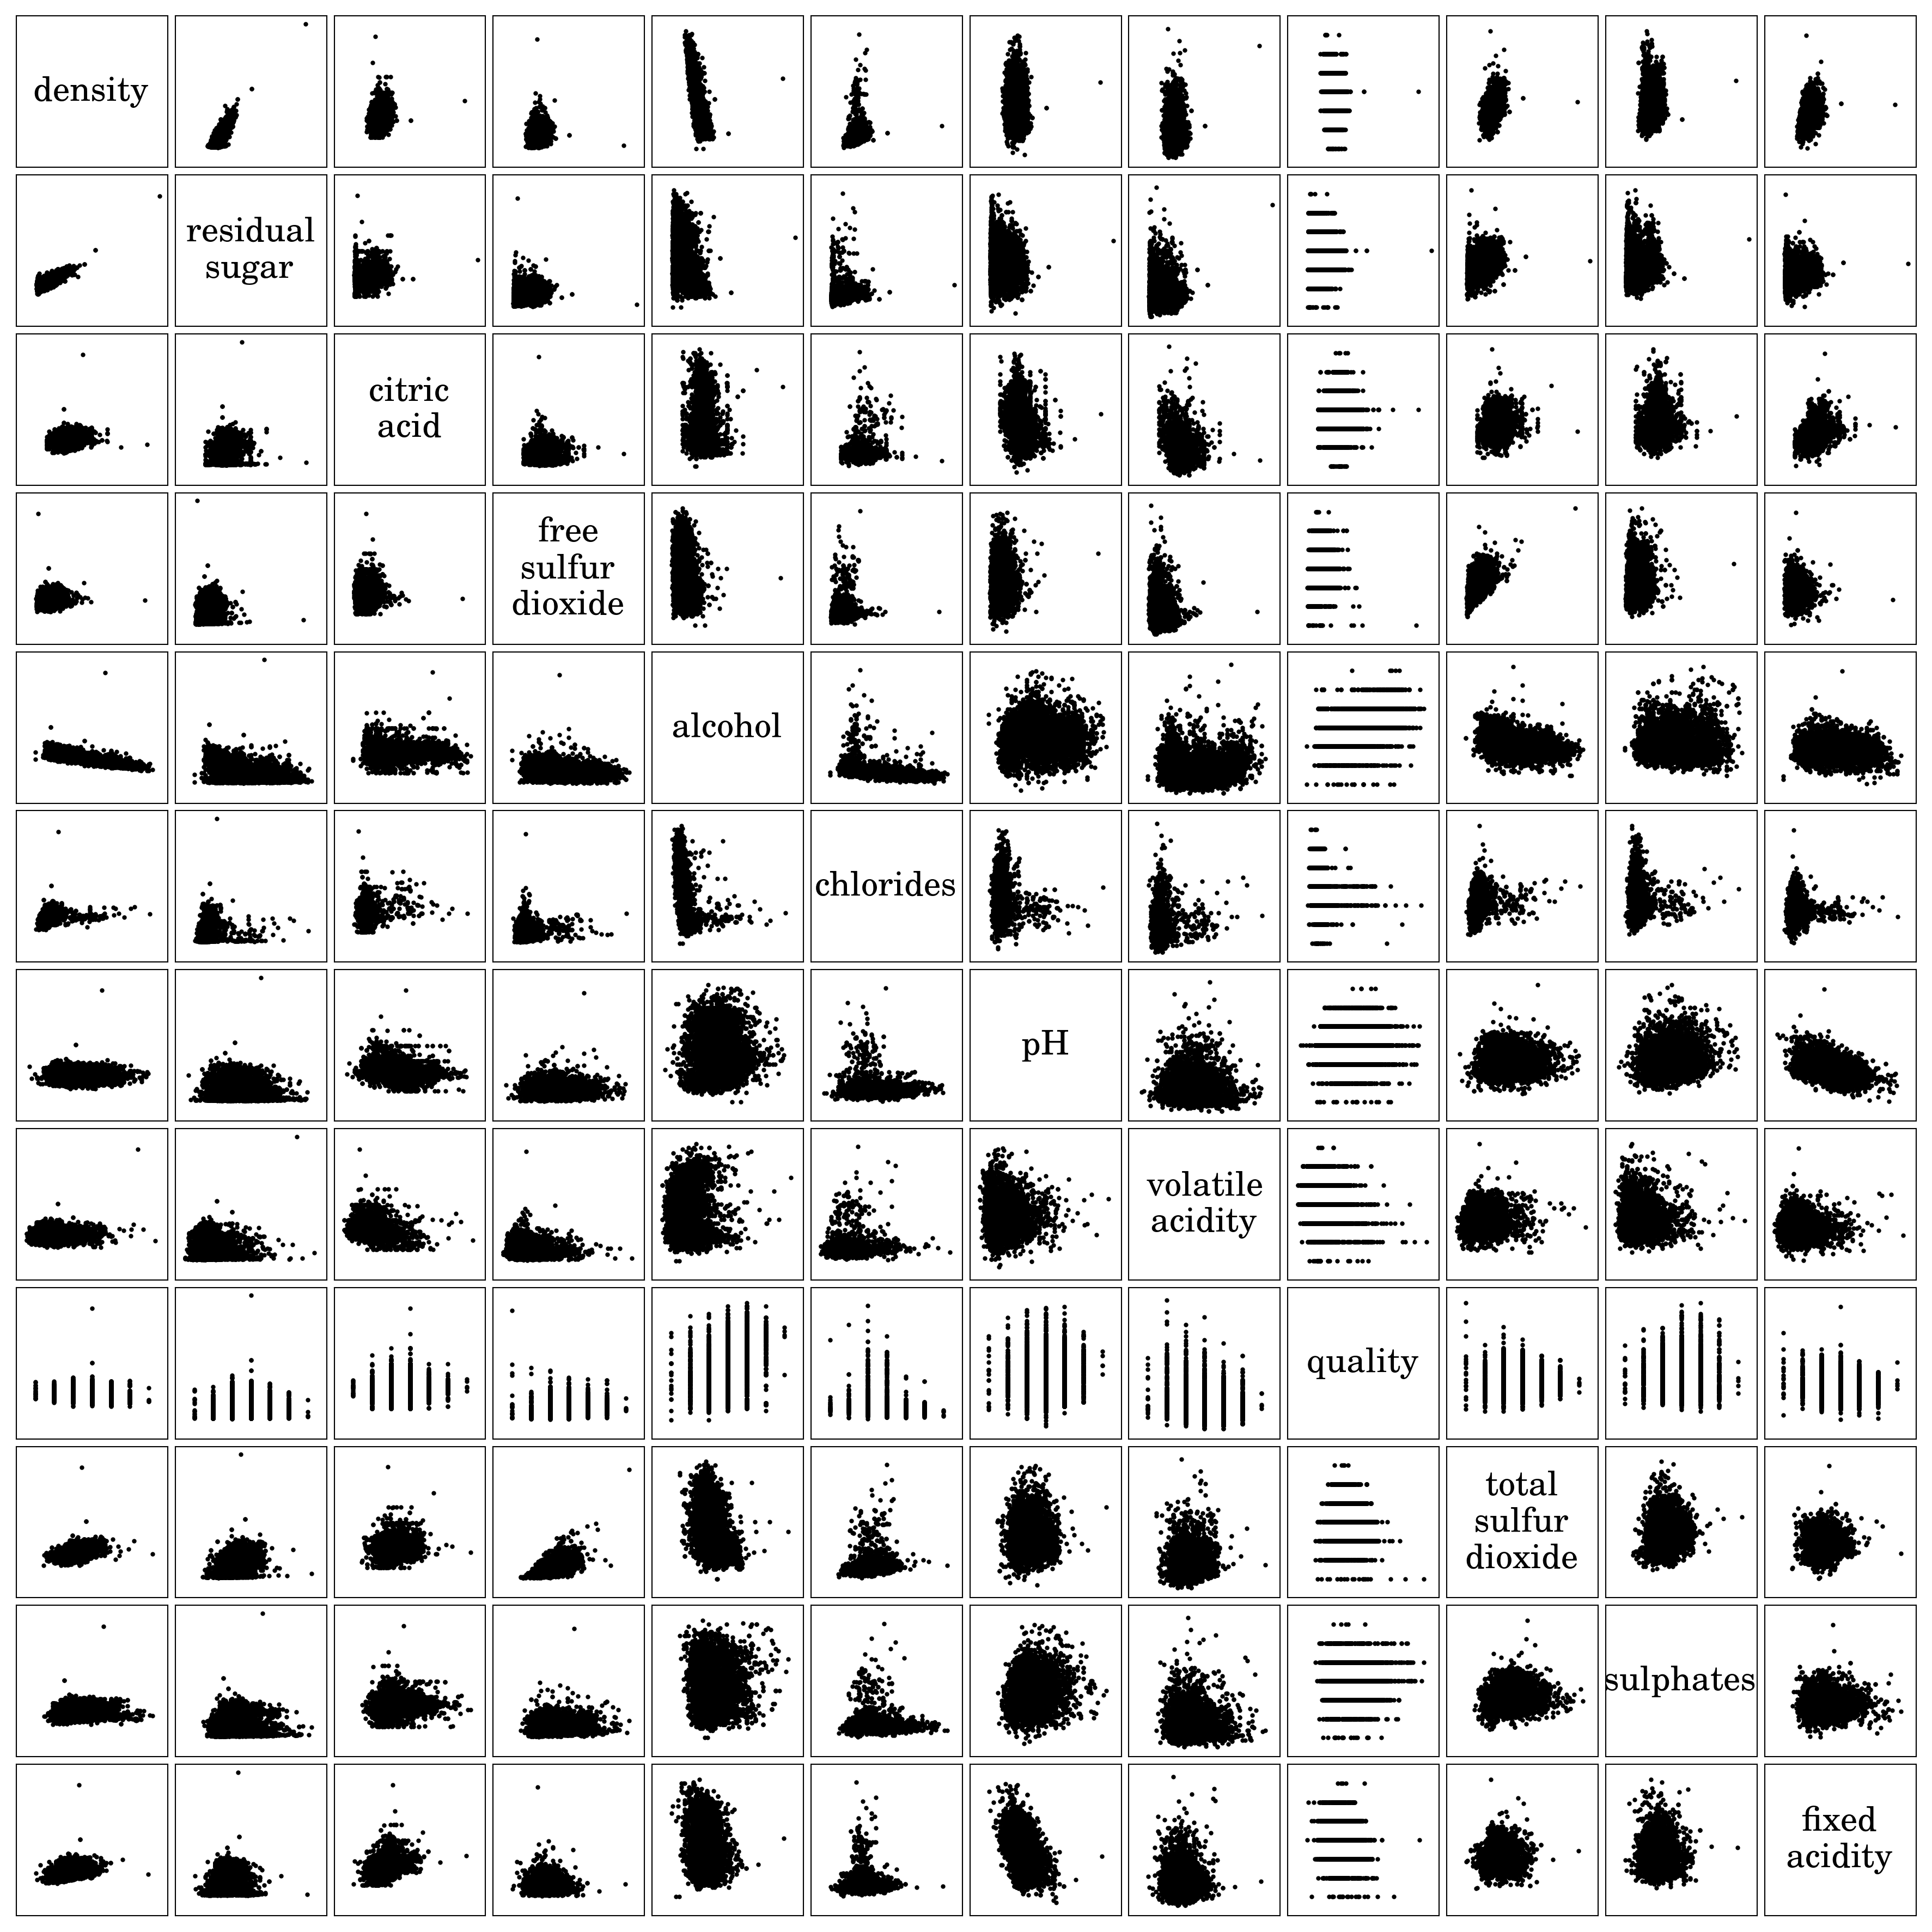
\includegraphics[width=\textwidth]{scattermatrix.png}
\caption{Scatter matrix of the whole feature set}
\end{figure}

\begin{figure}[H]
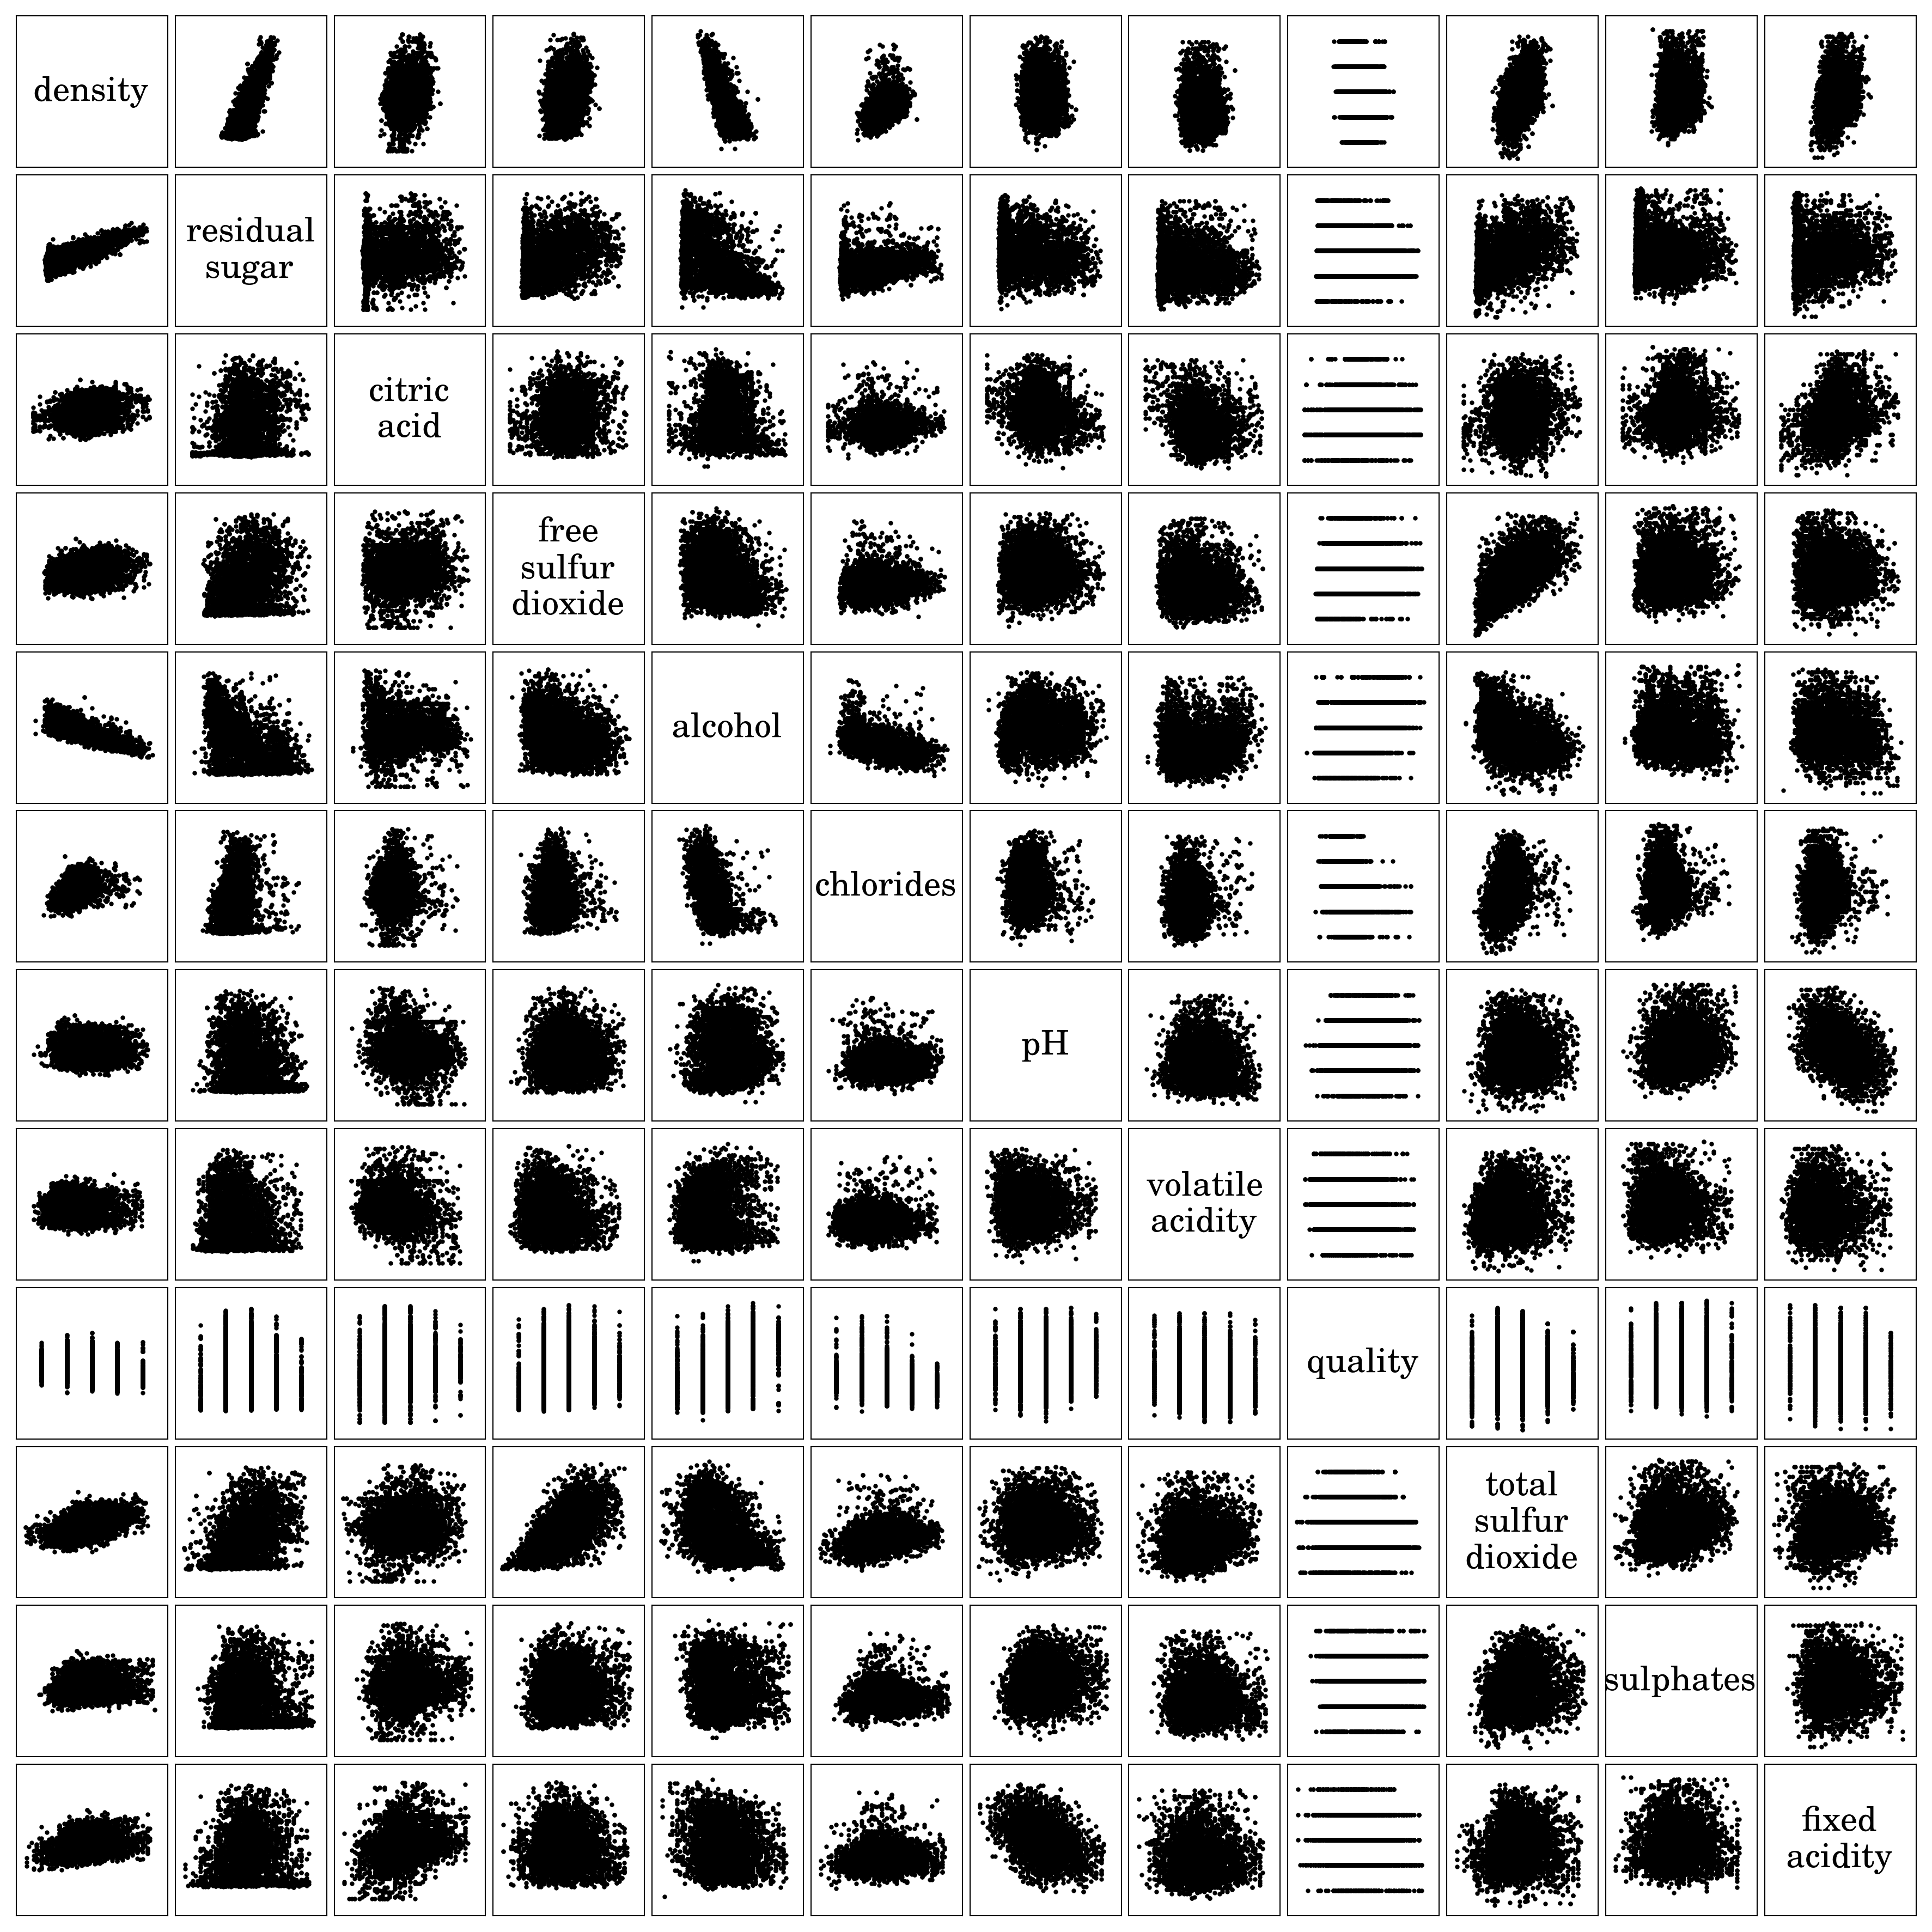
\includegraphics[width=\textwidth]{scattermatrix_filtered.png}
\caption{Scatter matrix of the whole feature set with outliers further than 3 standard deviations from the mean filtered}
\end{figure}

\begin{figure}[H]
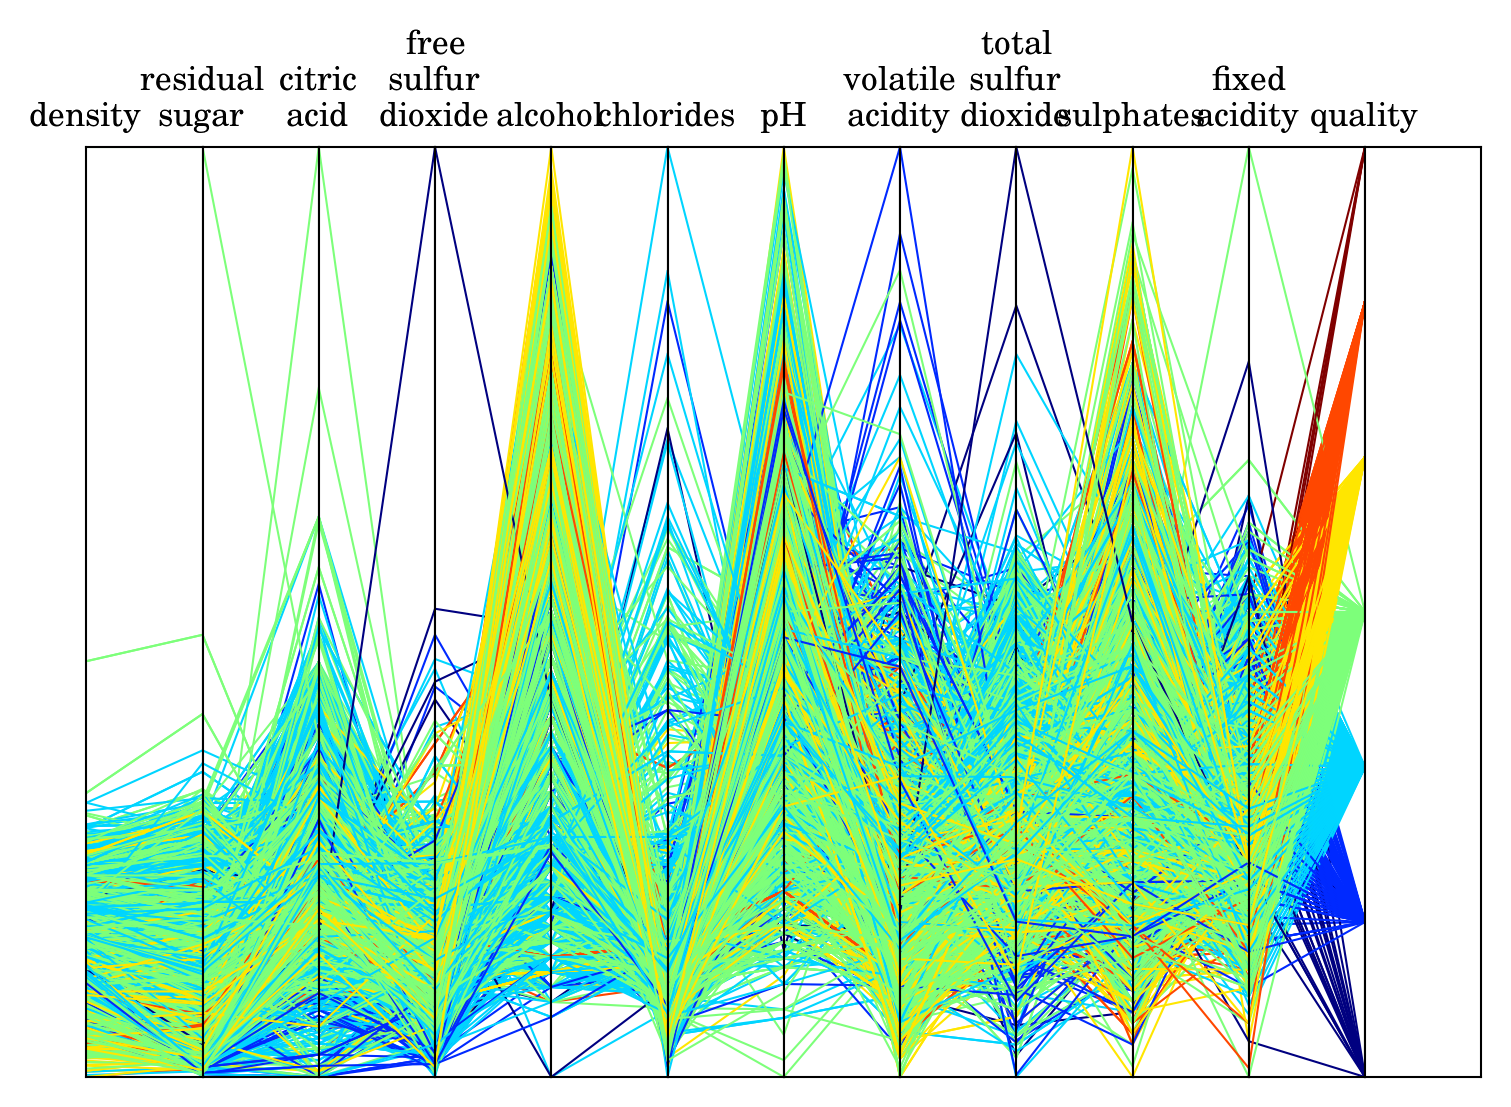
\includegraphics[width=\textwidth]{parallel_coords.png}
\caption{Parallel coordinates representation of the data set}
\end{figure}

\subsection{Principal component analysis}
\begin{figure}[H]
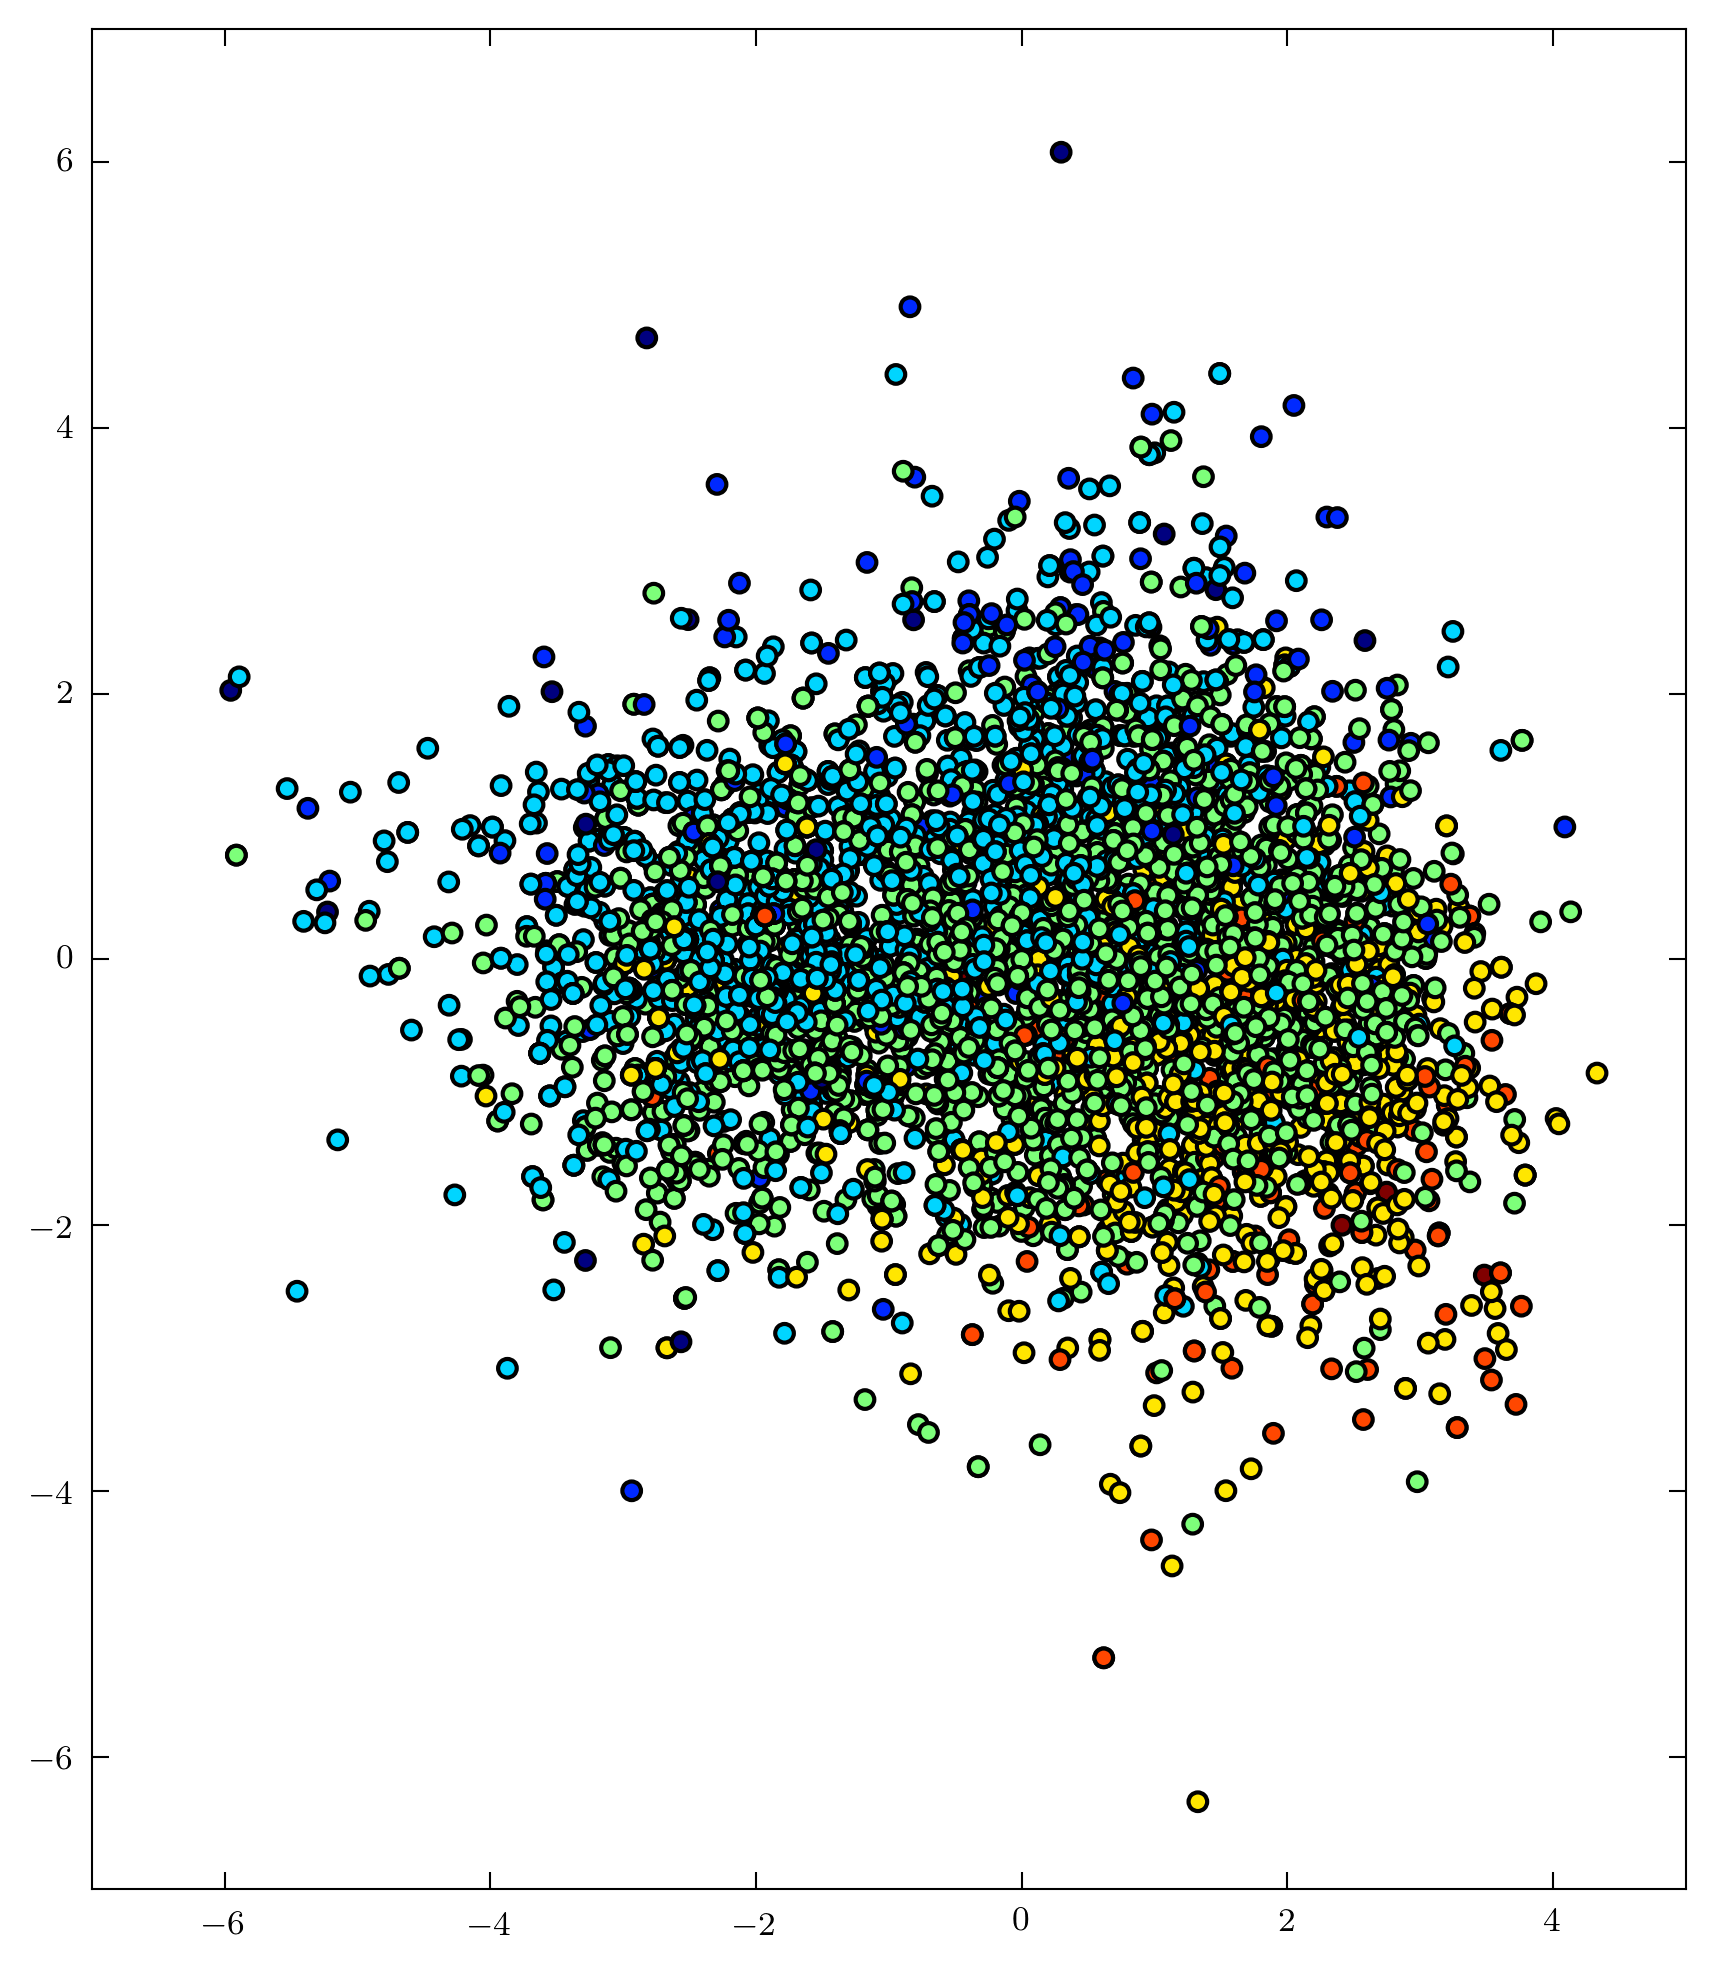
\includegraphics[width=\textwidth]{pca.png}
\caption{2D projection of the normalized data set using PCA}\end{figure}

\begin{adjustbox}{max width=\textwidth}
\begin{tabular}{l || *{13}{r}}
 & PC1 & PC2 & PC3 & PC4 & PC5 & PC6 & PC7 & PC8 & PC9 & PC10 & PC11 & PC12\\
\hline \\Proportion of variance & 0.2746 & 0.1317 & 0.1170 & 0.0923 & 0.0856 & 0.0746 & 0.0654 & 0.0581 & 0.0469 & 0.0293 & 0.0226 & 0.0017\\
Cumulative variance &0.2746 & 0.4063 & 0.5234 & 0.6157 & 0.7013 & 0.7760 & 0.8414 & 0.8995 & 0.9464 & 0.9757 & 0.9983 & 1.0000\\
\end{tabular}
\end{adjustbox}
\section{Correlation coefficients using different functions}

\subsection{Correlation coefficients using Pearson's correlation coefficient}
\begin{adjustbox}{max width=\textwidth}
\begin{tabular}{l || *{12}{P{1.2cm}}}
& residual sugar & fixed acidity & density & volatile acidity & total sulfur dioxide & alcohol & quality & sulphates & free sulfur dioxide & chlorides & citric acid & pH\\
\hline 
residual sugar & \bftab 1.0000 & 0.0890 & \bftab 0.8390 & 0.0643 & 0.4014 & --0.4506 & --0.0976 & --0.0267 & 0.2991 & 0.0887 & 0.0942 & --0.1941 \\

fixed acidity & 0.0890 & \bftab 1.0000 & 0.2653 & --0.0227 & 0.0911 & --0.1209 & --0.1137 & --0.0171 & --0.0494 & 0.0231 & 0.2892 & --0.4259 \\

density & \bftab 0.8390 & 0.2653 & \bftab 1.0000 & 0.0271 & \bftab 0.5299 & \bftab --0.7801 & --0.3071 & 0.0745 & 0.2942 & 0.2572 & 0.1495 & --0.0936 \\

volatile acidity & 0.0643 & --0.0227 & 0.0271 & \bftab 1.0000 & 0.0893 & 0.0677 & --0.1947 & --0.0357 & --0.0970 & 0.0705 & --0.1495 & --0.0319 \\

total sulfur dioxide & 0.4014 & 0.0911 & \bftab 0.5299 & 0.0893 & \bftab 1.0000 & --0.4489 & --0.1747 & 0.1346 & \bftab 0.6155 & 0.1989 & 0.1211 & 0.0023 \\

alcohol & --0.4506 & --0.1209 & \bftab --0.7801 & 0.0677 & --0.4489 & \bftab 1.0000 & 0.4356 & --0.0174 & --0.2501 & --0.3602 & --0.0757 & 0.1214 \\

quality & --0.0976 & --0.1137 & --0.3071 & --0.1947 & --0.1747 & 0.4356 & \bftab 1.0000 & 0.0537 & 0.0082 & --0.2099 & --0.0092 & 0.0994 \\

sulphates & --0.0267 & --0.0171 & 0.0745 & --0.0357 & 0.1346 & --0.0174 & 0.0537 & \bftab 1.0000 & 0.0592 & 0.0168 & 0.0623 & 0.1560 \\

free sulfur dioxide & 0.2991 & --0.0494 & 0.2942 & --0.0970 & \bftab 0.6155 & --0.2501 & 0.0082 & 0.0592 & \bftab 1.0000 & 0.1014 & 0.0941 & --0.0006 \\

chlorides & 0.0887 & 0.0231 & 0.2572 & 0.0705 & 0.1989 & --0.3602 & --0.2099 & 0.0168 & 0.1014 & \bftab 1.0000 & 0.1144 & --0.0904 \\

citric acid & 0.0942 & 0.2892 & 0.1495 & --0.1495 & 0.1211 & --0.0757 & --0.0092 & 0.0623 & 0.0941 & 0.1144 & \bftab 1.0000 & --0.1637 \\

pH & --0.1941 & --0.4259 & --0.0936 & --0.0319 & 0.0023 & 0.1214 & 0.0994 & 0.1560 & --0.0006 & --0.0904 & --0.1637 & \bftab 1.0000 \\
\end{tabular}
\end{adjustbox}
\subsection{Correlation coefficients using Spearman's rho}
\begin{adjustbox}{max width=\textwidth}
\begin{tabular}{l || *{12}{P{1.2cm}}}
& residual sugar & fixed acidity & density & volatile acidity & total sulfur dioxide & alcohol & quality & sulphates & free sulfur dioxide & chlorides & citric acid & pH\\
\hline 
residual sugar & \bftab 1.0000 & 0.1067 & \bftab 0.7804 & 0.1086 & 0.4313 & --0.4453 & --0.0821 & --0.0038 & 0.3461 & 0.2278 & 0.0246 & --0.1800 \\

fixed acidity & 0.1067 & \bftab 1.0000 & 0.2700 & --0.0429 & 0.1126 & --0.1068 & --0.0845 & --0.0132 & --0.0245 & 0.0947 & 0.2979 & --0.4183 \\

density & \bftab 0.7804 & 0.2700 & \bftab 1.0000 & 0.0101 & \bftab 0.5638 & \bftab --0.8219 & --0.3484 & 0.0951 & 0.3278 & \bftab 0.5083 & 0.0914 & --0.1101 \\

volatile acidity & 0.1086 & --0.0429 & 0.0101 & \bftab 1.0000 & 0.1176 & 0.0340 & --0.1966 & --0.0169 & --0.0812 & --0.0049 & --0.1504 & --0.0452 \\

total sulfur dioxide & 0.4313 & 0.1126 & \bftab 0.5638 & 0.1176 & \bftab 1.0000 & --0.4766 & --0.1967 & 0.1578 & \bftab 0.6186 & 0.3752 & 0.0932 & --0.0118 \\

alcohol & --0.4453 & --0.1068 & \bftab --0.8219 & 0.0340 & --0.4766 & \bftab 1.0000 & 0.4404 & --0.0449 & --0.2726 & \bftab --0.5708 & --0.0292 & 0.1489 \\

quality & --0.0821 & --0.0845 & --0.3484 & --0.1966 & --0.1967 & 0.4404 & \bftab 1.0000 & 0.0333 & 0.0237 & --0.3145 & 0.0183 & 0.1094 \\

sulphates & --0.0038 & --0.0132 & 0.0951 & --0.0169 & 0.1578 & --0.0449 & 0.0333 & \bftab 1.0000 & 0.0523 & 0.0939 & 0.0798 & 0.1402 \\

free sulfur dioxide & 0.3461 & --0.0245 & 0.3278 & --0.0812 & \bftab 0.6186 & --0.2726 & 0.0237 & 0.0523 & \bftab 1.0000 & 0.1670 & 0.0883 & --0.0063 \\

chlorides & 0.2278 & 0.0947 & \bftab 0.5083 & --0.0049 & 0.3752 & \bftab --0.5708 & --0.3145 & 0.0939 & 0.1670 & \bftab 1.0000 & 0.0327 & --0.0540 \\

citric acid & 0.0246 & 0.2979 & 0.0914 & --0.1504 & 0.0932 & --0.0292 & 0.0183 & 0.0798 & 0.0883 & 0.0327 & \bftab 1.0000 & --0.1462 \\

pH & --0.1800 & --0.4183 & --0.1101 & --0.0452 & --0.0118 & 0.1489 & 0.1094 & 0.1402 & --0.0063 & --0.0540 & --0.1462 & \bftab 1.0000 \\
\end{tabular}
\end{adjustbox}
\subsection{Correlation coefficients using Kendall's tau}
\begin{adjustbox}{max width=\textwidth}
\begin{tabular}{l || *{12}{P{1.2cm}}}
& residual sugar & fixed acidity & density & volatile acidity & total sulfur dioxide & alcohol & quality & sulphates & free sulfur dioxide & chlorides & citric acid & pH\\
\hline 
residual sugar & \bftab 1.0000 & 0.0749 & \bftab 0.5890 & 0.0728 & 0.2933 & --0.3056 & --0.0631 & --0.0025 & 0.2367 & 0.1553 & 0.0153 & --0.1256 \\

fixed acidity & 0.0749 & \bftab 1.0000 & 0.1855 & --0.0296 & 0.0773 & --0.0732 & --0.0655 & --0.0087 & --0.0169 & 0.0654 & 0.2086 & --0.2948 \\

density & \bftab 0.5890 & 0.1855 & \bftab 1.0000 & 0.0066 & 0.3884 & \bftab --0.6351 & --0.2666 & 0.0642 & 0.2173 & 0.3491 & 0.0615 & --0.0756 \\

volatile acidity & 0.0728 & --0.0296 & 0.0066 & \bftab 1.0000 & 0.0813 & 0.0235 & --0.1548 & --0.0116 & --0.0548 & --0.0035 & --0.1040 & --0.0304 \\

total sulfur dioxide & 0.2933 & 0.0773 & 0.3884 & 0.0813 & \bftab 1.0000 & --0.3258 & --0.1512 & 0.1087 & 0.4447 & 0.2571 & 0.0622 & --0.0084 \\

alcohol & --0.3056 & --0.0732 & \bftab --0.6351 & 0.0235 & --0.3258 & \bftab 1.0000 & 0.3467 & --0.0264 & --0.1825 & --0.4040 & --0.0200 & 0.1026 \\

quality & --0.0631 & --0.0655 & --0.2666 & --0.1548 & --0.1512 & 0.3467 & \bftab 1.0000 & 0.0264 & 0.0172 & --0.2449 & 0.0146 & 0.0844 \\

sulphates & --0.0025 & --0.0087 & 0.0642 & --0.0116 & 0.1087 & --0.0264 & 0.0264 & \bftab 1.0000 & 0.0356 & 0.0626 & 0.0545 & 0.0958 \\

free sulfur dioxide & 0.2367 & --0.0169 & 0.2173 & --0.0548 & 0.4447 & --0.1825 & 0.0172 & 0.0356 & \bftab 1.0000 & 0.1139 & 0.0608 & --0.0052 \\

chlorides & 0.1553 & 0.0654 & 0.3491 & --0.0035 & 0.2571 & --0.4040 & --0.2449 & 0.0626 & 0.1139 & \bftab 1.0000 & 0.0223 & --0.0379 \\

citric acid & 0.0153 & 0.2086 & 0.0615 & --0.1040 & 0.0622 & --0.0200 & 0.0146 & 0.0545 & 0.0608 & 0.0223 & \bftab 1.0000 & --0.1013 \\

pH & --0.1256 & --0.2948 & --0.0756 & --0.0304 & --0.0084 & 0.1026 & 0.0844 & 0.0958 & --0.0052 & --0.0379 & --0.1013 & \bftab 1.0000 \\
\end{tabular}
\end{adjustbox}
\end{document}